\documentclass[10pt,a4paper,ngerman]{article}
\usepackage[margin=2.5cm]{geometry}
\usepackage[T1]{fontenc}
\usepackage[utf8]{inputenc} % Zeichensatz
\usepackage[ngerman]{babel} % Sprachpaket
\usepackage{amsmath}  % Mathematik
\usepackage{amsfonts} % Mathematik
\usepackage{amssymb}  % Mathematik
\usepackage{palatino} % Schriftart
\usepackage{titling}  % für eigene Überschrift
\usepackage{graphicx}
\usepackage{subcaption}
\usepackage{wasysym}  % enthält Symbole, wie Quadrate (für Multiple Choice Fragen)
\usepackage{dirtree}  % Verzeichnisbäume
\usepackage{hyperref} % Hyperlinks und andere Verlinkungen

% Package für die Kopf- und Fußzeilen
\usepackage{scrlayer-scrpage}
\pagestyle{scrheadings}
\clearpairofpagestyles % Die einzelnen Bereiche leeren

% Quelltext-Listings 
\usepackage{listings} % Listings
\usepackage{color}    % Syntax-Highlighting

% Farben definieren (für Syntax-Highlighting)
\definecolor{middlegray}{rgb}{0.5,0.5,0.5}
\definecolor{lightgray}{rgb}{0.8,0.8,0.8}
\definecolor{darkgray}{gray}{0.2} % gray: nur ein Wert wird angegeben, welcher dem Grauton entspricht
\definecolor{comment}{rgb}{0.0,0.5,0.0}
\definecolor{keywordcolor}{rgb}{0.0, 0.28, 0.67}

\newcommand{\lstfs}{\fontsize{10}{12}}

% Listings formatieren
\lstset{
   	basicstyle=\ttfamily\lstfs,
   	keywordstyle=\bfseries\ttfamily\color{keywordcolor},
   	stringstyle=\color{darkgray}\ttfamily,
   	commentstyle=\color{comment}\ttfamily,
  	emph={square}, 
   	emphstyle=\ttfamily,
   	emph={[2]root,base},
   	emphstyle={[2]\ttfamily},
   	showstringspaces=false,
   	flexiblecolumns=false,
   	tabsize=2,
   	numbers=left,
   	numberstyle=\tiny,
   	numberblanklines=false,
   	stepnumber=5,
   	firstnumber=1,
 	numberfirstline=true,
   	numbersep=10pt,
	xleftmargin=15pt,
	literate={ö}{{\"o}}1
           {ä}{{\"a}}1
           {ü}{{\"u}}1
           {ß}{{\ss}}1
}



% Metainformationen
\title{Evaluation -- Praktikum 3}
\author{Die Lokalisatoren}

\ihead{}
\chead{}
\ohead{}
\ifoot{}
\cfoot{\pagemark}
\ofoot{}


\newcommand{\doctitle}[1]{\begin{center}\begin{huge}#1\end{huge}\end{center}}

% 1. Variante des docheader (ohne Parameter)
% dann wird der Autor unter der Überschrift ausgegeben
\newcommand{\docheader}{\doctitle{\thetitle}\begin{center}\theauthor\end{center}\hrule\vspace{1em}}

% 2. Variante des docheader (mit Parameter)
% was im Parameter steht wird unter der Überschrift ausgeben
\newcommand{\docheaderparam}[1]{\doctitle{\thetitle}\begin{center}#1\end{center}\hrule\vspace{1em}}

\newcommand{\timbox}[1]{\begin{center}\fbox{\begin{minipage}[t]{0.8\textwidth}#1\end{minipage}}\end{center}}

\newcommand{\code}[1]{\texttt{#1}}

% Für Multiple Choice
\newcommand{\choice}{\item[\Square]}
\newcommand{\cchoice}{\item[\CheckedBox]} % cc = correc choice

\setlength{\parskip}{0em}
\setlength{\parindent}{0em}
\renewcommand{\baselinestretch}{1.5}

\begin{document}

\begin{figure}[t]
	\flushright
	
\includegraphics[width=5cm]{hs-bo-logo}
\end{figure}

\docheader

\section{Technische Umsetzung}
Die Applikation baut auf der in den ersten beiden Praktika entwickelten App auf. Dadurch war schon eine Grundstruktur, mit z.B. Einstellungen für die Serververbindung und der Berechtigungsabfrage gegeben.
Es wurden zwei zusätzliche Aktivitäten hinzugefügt, eine zur GPS-Messung mit einer periodischen Reportingstrategie und eine mit Distanz-basierter Reportingstrategie.
Die periodische-Reportigstrategie fragt GPS Updates mit dem zuvor eingestellten Zeitintervall an. Im optimalen Fall ruft die Betriebssystem API nun in genau diesem Intervall die Callbackfunktion auf. In dieser Funktion wird das Location Objekt zwischen gespeichert und die POST-Anfrage an den Server gestellt. Die Aktivität der periodischen Reportingstrategie bietet zudem einen Button, mit dem eine POST Anfrage an den API-Endpunkt gesendet wird, durch den der Export der in der Datenbank gesammelten Daten in eine KML-Datei angestoßen wird.

Die Aktivität der  Distanz-basierten Reportingstrategie baut auf der Aktivität der periodischen Reportingstrategie auf. Hier wurde die Anfrage der GPS Updates geändert, so dass das Zeitintervall auf Null Sekunden gestellt wurde. Durch diese Änderung wird die Callbackfunktion aufgerufen, sobald ein neues Positionsupdate vorliegt. In dieser Callbackfunktion werden die Positionsupdates mit der zuletzt gemessenen Position verglichen. In dem Fall, dass der Abstand der beiden Positionen größer ist als die zuvor festgelegte Distanz, wird die neue Position zwischengespeichert und an den Server gesendet.
Die geschwindigkeitsabhängige Strategie wurde mit Hilfe eines Handlers implementiert, der nach der errechneten Zeit, die voraussichtlich für die Strecke benötigt wird, die GPS abfrage wieder startet.
Die bewegungsabhängige Strategie ermittelt mit Hilfe des Accelerometers wie groß die momentane Beschleunigung des Gerätes in alle drei Achsen ist. Übersteigt eine von ihnen $5m/s^2$ oder $-5m/s^2$ wird die GPS Abfrage wieder gestartet.

Der Server wurde mit Node.js umgesetzt, die empfangenen Daten werden in einer MongoDB abgespeichert. Der Server bietet die Funktionen Daten über eine API zusenden und über eine POST anfrage an einen API Endpunkt den Exportprozess der Daten in eine KML-Datei zu starten.

\section{Aufbau und Ablauf der Messung}
Die Messung fanden in der Umgebung der Siedlung Am Stenshof in Bochum statt. Die Messroute wurde zu Fuß abgegangen und beträgt ungefähr 950 Meter. Mit einer 30 Sekunden langen und einer 60 Sekunden langen Pause beträgt die Dauer einer Messung ungefähr zehn bis zwölf Minuten.

Es wurden Messungen mit vier verschiedenen Reportingstrategien durch geführt:
\begin{enumerate}
	\item{Periodische Reportingstrategie mit einem Zeitintervall von einer Sekunde}
	\item{Distanz-basierte Reportingstrategie mit einem Abstand von 50 Metern}
	\item{Geschwindigkeis und Distanz-basierte Reportingstrategie mit einem Abstand von 50 Metern und einer maximalen Geschwindigkeit von 2 m/s}
	\item{Bewegungsb-bewusste Distanz-basierte Reportingstrategie mit einem Abstand von 50 Metern}
\end{enumerate}

\section{Erwartungen}

\subsection{Periodische Reportingstrategie}
Bei der Periodischen Reportingstrategie ist zu erwarten, dass der Streckenverlauf anhand der gespeicherten Positionsfixes sehr gut nachzuvollziehen sein wird. Zudem werden bei Pausen mehrere Fixes auf einer Stelle sein. Die Anzahl der Serverseitig empfangenen Positionen sollte mit der Anzahl der Positionen die das Gerät empfangen hat übereinstimmen.

\subsection{Distanz-basierte Reportingstrategie}
Bei der Distanz-basierten Strategie werden im Vergleich zu der periodischen Strategie vorraussichtlich deutlich weniger Fixes auf dem Server gespeichert. Zu dem wird durch die geringere Anzahl der Fixes die abgelaufene Route schlechter zu erkennen sein. Serverseitig sollten deutlich weniger Positionen erfasst werden, als auf dem Gerät.

\subsection{Geschwindigkeits und Distanz-basierte Reportingstrategie}
Bei der Geschwindigkeits und Distanz-basierten Strategie wird die Anzahl der Fixes der der Distanz-basierten Strategie ungefähr gleichen. Serverseitig sollten deutlich weniger Positionen erfasst werden, als auf dem Gerät.

\subsection{Distanz-basierte Reportingstrategie mit Bewegungserkennung}
Bei dieser Strategie ist davon auszugehen, dass die Anazahl der Fixes wieder ungefähr der Anzahl der anderen Distanz-basierten Strategien gleicht. Serverseitig sollten deutlich weniger Positionen erfasst werden, als auf dem Gerät.

\section{Auswertung}
Zu Beginn jeder Messung sind bei dem ersten Positionsfix erhebliche Positionsfehler erkennbar. 

\subsection{Periodische Reportingstrategie}
Wie angenommen ist der Streckenverlauf sehr detailliert aufgezeichnet worden (759 Punkte). Auffällig ist der zweite Positionsfix, dieser hat einen Abstand von zirka 70 Metern zum ersten und dritten Fix. Im gesamten folgenden Verlauf der Messung sind keine derartigen Ausreißer erkennbar. Außerdem auffällig sind die Positionsfixes während der Pausen. Dort sind kleine Spitzen erkennbar, obwohl die Pausen direkt auf der Messstrecke eingelegt worden sind (Siehe Abb. 3 und 4).

\subsection{Distanz-basierte Reportingstrategie}
Hier sind wie erwartet deutlich weniger Positionsfixes auf dem Server gespeichert worden (0,031 Uplink/s gegenüber 1 Uplink/s). Durch die geringere Anzahl der Fixes ist mit Hilfe der Daten nur noch eine Approximation an die Ursprüngliche Route möglich. Hervor sticht, dass die ersten neun Positionsfixe deutlich neben der Messstrecke liegen. Dadurch kann der Wert der Uplink/s verfälscht werden. Zum Beispiel wenn die GPS Position so weit von der eigentlichen Position abweicht, dass diese Position gesendet wird.

\subsection{Geschwindigkeits und Distanz-basierte Reportingstrategie}
Wie vermutet, ist bei dieser Strategie eine ähnliche Anzahl an Fixes auf dem Server gespeichert worden wie bei der zweiten Route. Die Uplinks pro Sekunde stimmen sogar gerundet überein. Im Gegensatz dazu, hat das Gerät bei dieser Strategie deutlich weniger GPS Updates erhalten (0,207 GPS-F/s gegenüber 0,999 GPS-F/s). Dies ist darauf zurück zuführen, dass diese Strategie den Stromverbrauch optimiert, aber vor erreichen des konfigurierten Abstandes wieder GPS Fixes angefordert werden. Auch hier ist eine größere Anzahl von GPS Fehlern erkennbar. 

\subsection{Distanz-basierte Reportingstrategie mit Bewegungserkennung}
Die Anzahl der Fixes die an den Server gesendet wurden bleibt zu den beiden voran gegangen Strategien ähnlich (0,021 Uplink/s). Die bei den zwei vorherigen Strategien erkennbaren Fehler sind bei dieser Messung nicht erkennbar. Hier sind nur zu Beginn der Messung zwei größere GPS Fehler erkennbar, die restlichen Positionsfixe liegen sehr nah am ursprünglichen Streckenverlauf. Dadurch lässt sich vermutlich der etwas geringere Uplink/s-Wert erklären, da bei den anderen beiden Strategien durch die Fehler ungewollte zusätzliche Uplinks gesendet worden sind.

\section{Eignung der Strategien}
Die periodische Strategie eignet sich sehr gut, um sehr genaue Positionsverläufe zu dokumentieren. Sie eignet sich allerdings weniger für Backgroundservices oder Messungen über längere Zeiträume, da das GPS dauerhat eingeschaltet ist.\\
Der einzige Vorteil der zweiten Strategie liegt darin, dass die Positionsfixe gefiltert werden und somit weniger Daten verarbeitet werden müssen, falls eine nicht so hohe Auflösung zwischen den Fixes benötigt wird.\\
Die Geschwindigkeits-basierte Strategie hat gegenüber der rein Distanz-basierten Strategie den Vorteil, dass hier das GPS zwischenzeitlich abgeschaltet und somit der Akku weniger belastet wird. Diese Strategie sollte vor allem bei der Lokalisation in Fahrzeugen oder ähnlichem von Vorteil sein, da diese sich in der Regel mit recht konstanter Geschwindigkeit bewegen und die Geschwindigkeits-basierte Strategie die besten Ergebnisse bei einer konstanten Geschwindigkeit nahe der eingestellten maximal Geschwindigkeit erbringen sollte.\\
Die Bewegungs-basierte Strategie hat wie die Geschwindigkeits-basierte Strategie den Vorteil, dass er GPS Empfänger zwischendurch ausgeschaltet wird und dadurch der Akku weniger belastet wird. Allerdings sollte diese Strategie weniger für Fahrzeuge geeignet sein, da diese sich auch sehr ruhig und mit gleichbleibender Geschwindigkeit fortbewegen können und dort die Bewegungen dann zu schwach sein könnten um die Schwelle zu überschreiten ab der wieder GPS Fixe angefordert werden. Im Gegensatz dazu ist diese Strategie sehr gut für Fußgänger geeignet, da diese in der Regel recht große Unterschiede in den Beschleunigungswerten verursachen.

\section{Tabelle}

\centering
\begin{tabular}{llllll}
Strategie       & Anzahl Fixes & Anzahl Uplink & Zeitspanne                 & GPS-F / s & Uplink / s \\
Periodisch      & 759          & 759           & 17:50:12 - 18:02:51 (759s) & 1         & 1          \\
Distanz         & 734          & 23            & 19:44:45 - 19:57:00 (735s) & 0,999     & 0,031      \\
Geschwindigkeit & 173          & 26            & 20:07:27 - 20:21:24 (837s) & 0,207     & 0,031      \\
Bewegung        & 264          & 14            & 20:33:02 - 20:44:07 (665s) & 0,397     & 0,021    
\end{tabular}

\newpage
\section{Screenshots / Visualisierungen}

\begin{figure}[h!]
    \centering
    \begin{subfigure}[b]{0.35\textwidth}
        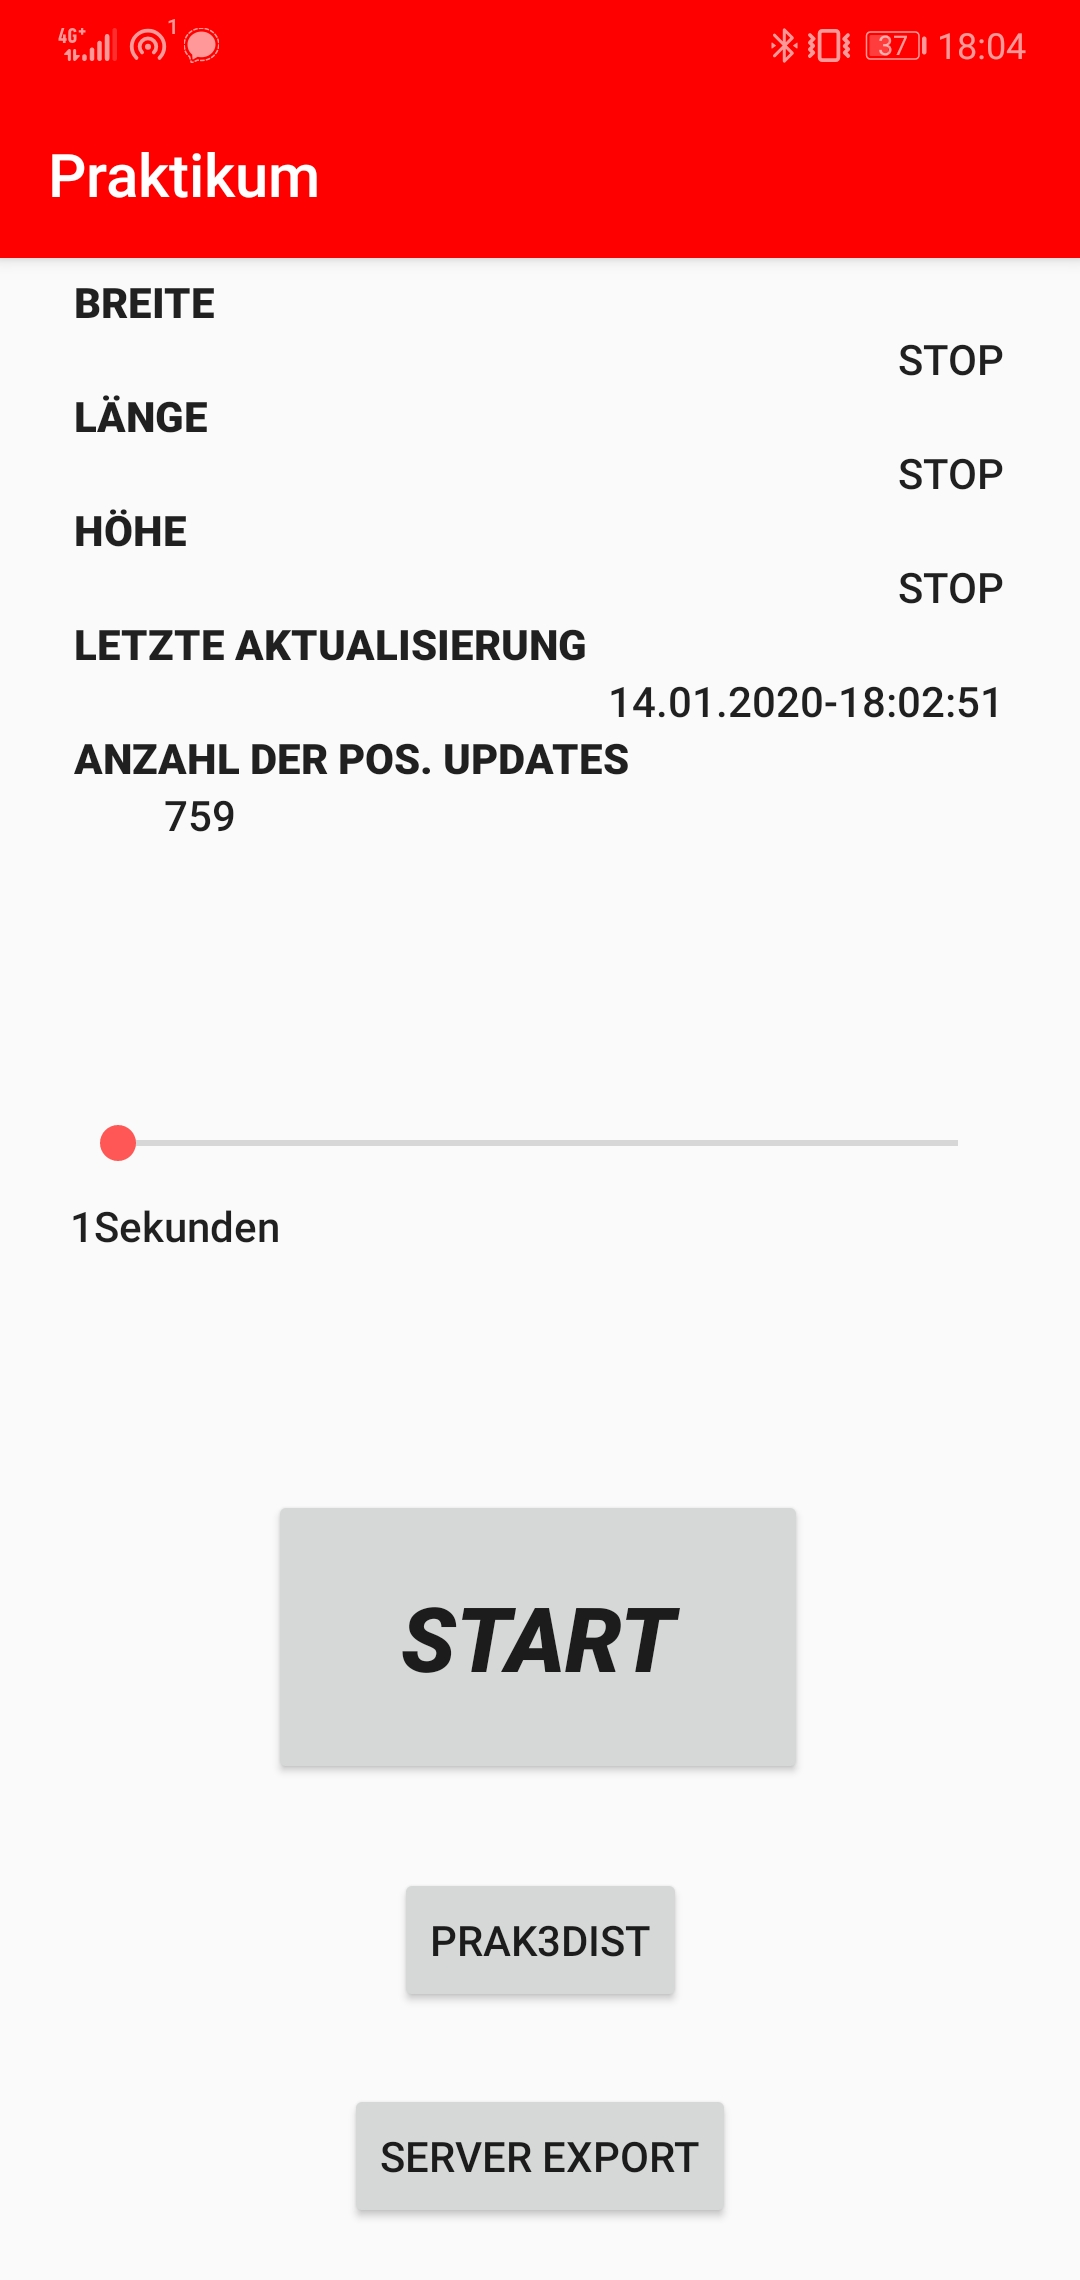
\includegraphics[width=\textwidth]{Screenshot_route1}
        \caption{GUI Periodische Reportingstrategie, nach der Messung}
        \label{fig:auswertung1}
    \end{subfigure}
    ~ % Abstand
    \begin{subfigure}[b]{0.35\textwidth}
        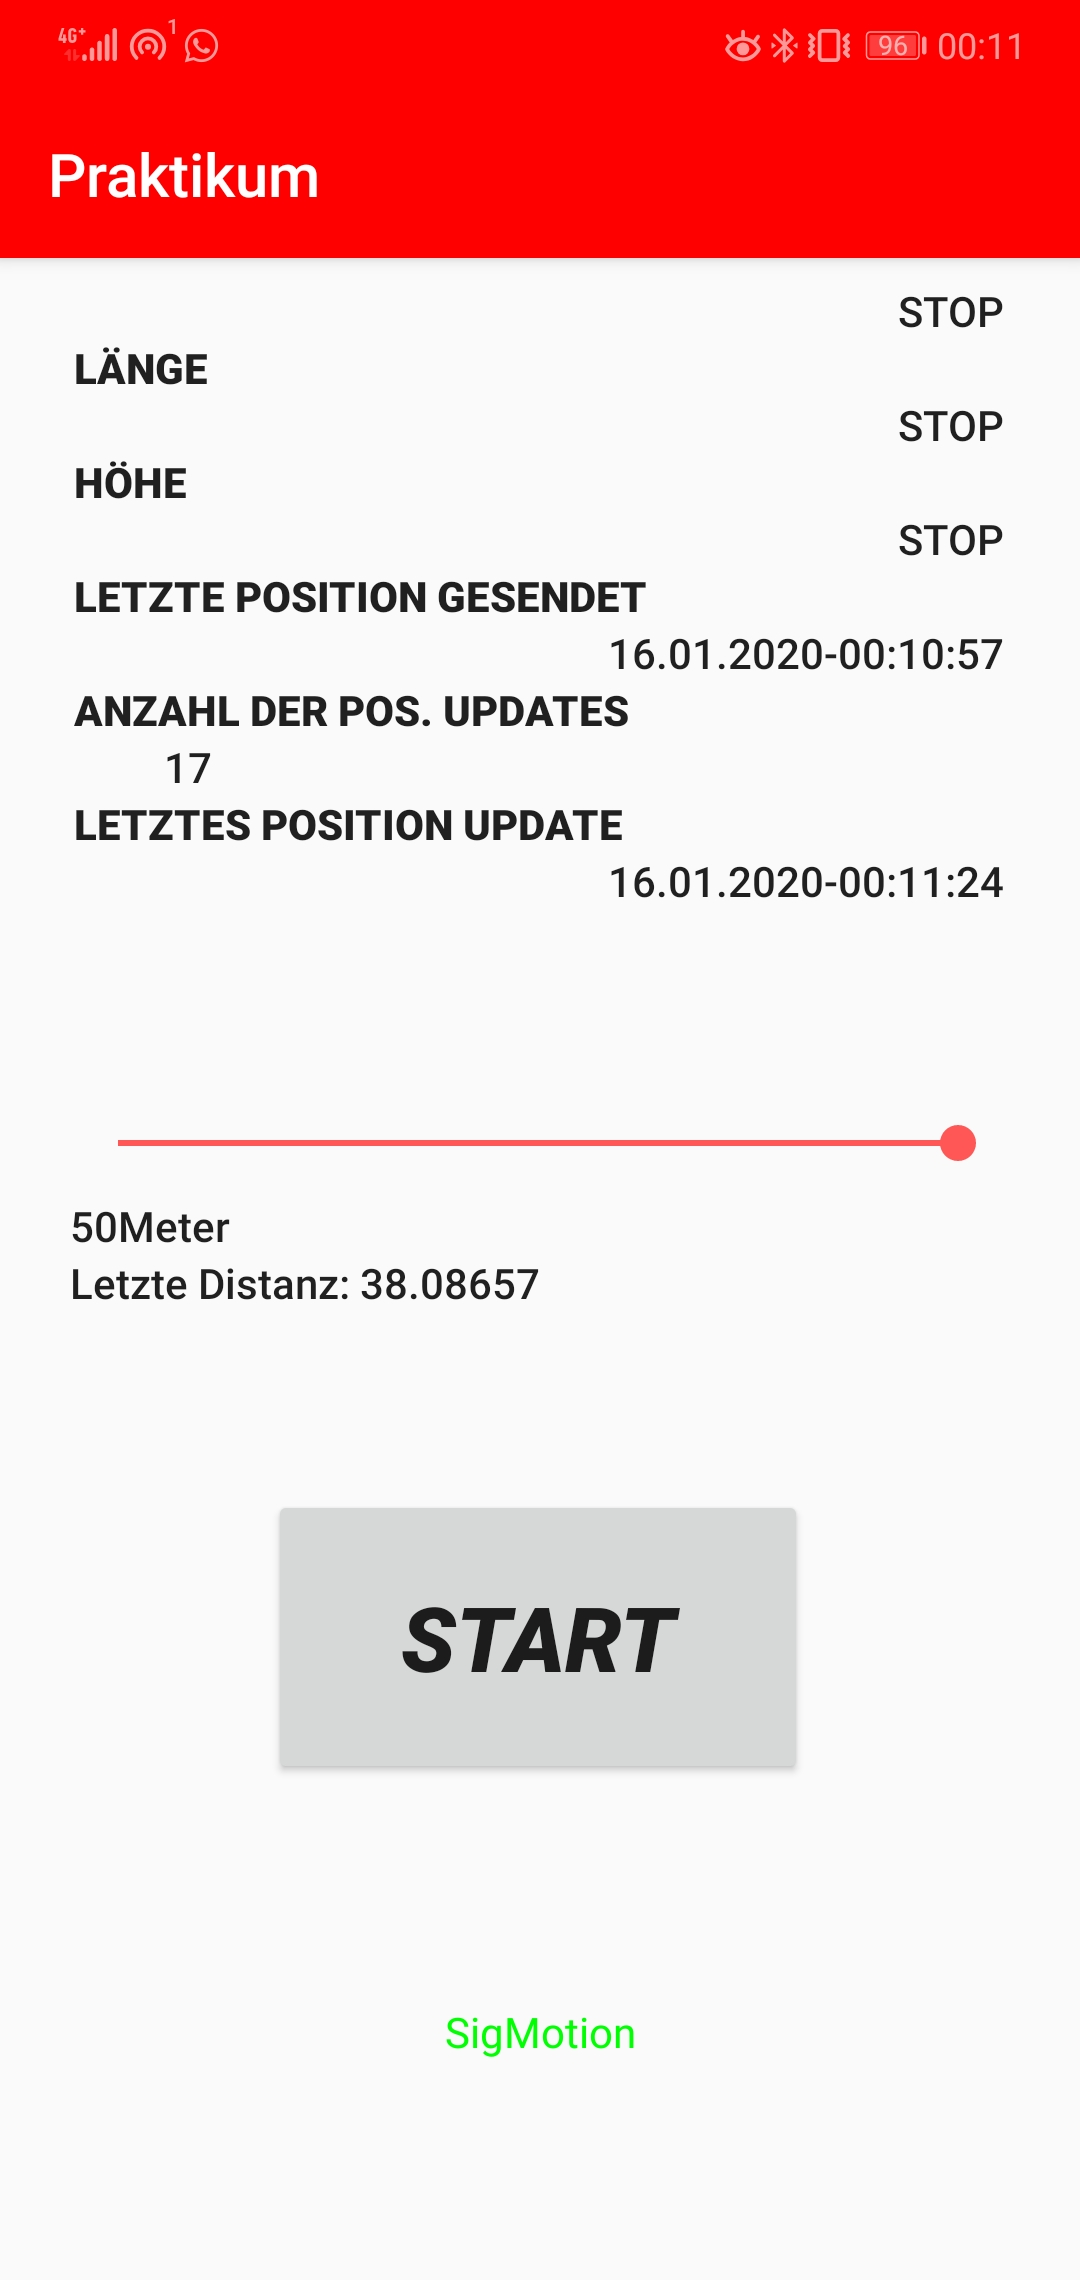
\includegraphics[width=\textwidth]{Screenshot_route2}
        \caption{GUI Distanz-basierte Reportingstrategie, nach der 2. Messung}
        \label{fig:auswertung2}
    \end{subfigure}
    \caption{Screenshots der beiden Aktivitäten Layouts}
    \label{fig:auswertung}
\end{figure}

\begin{figure}[h!]
    \centering
    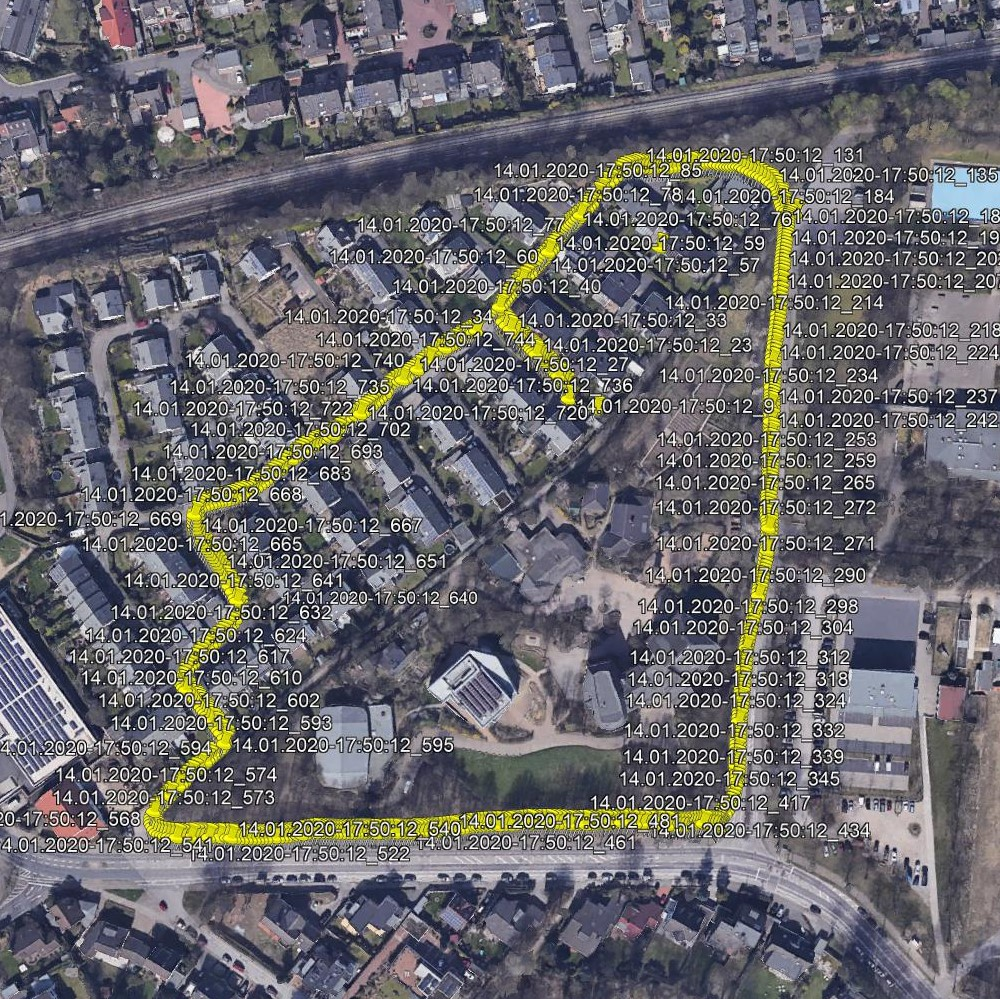
\includegraphics[width=0.8\textwidth]{Route1}
    \caption{Übersicht Fixes Messung 1}
    \label{fig:map}
\end{figure}
\begin{figure}[h!]
    \centering
    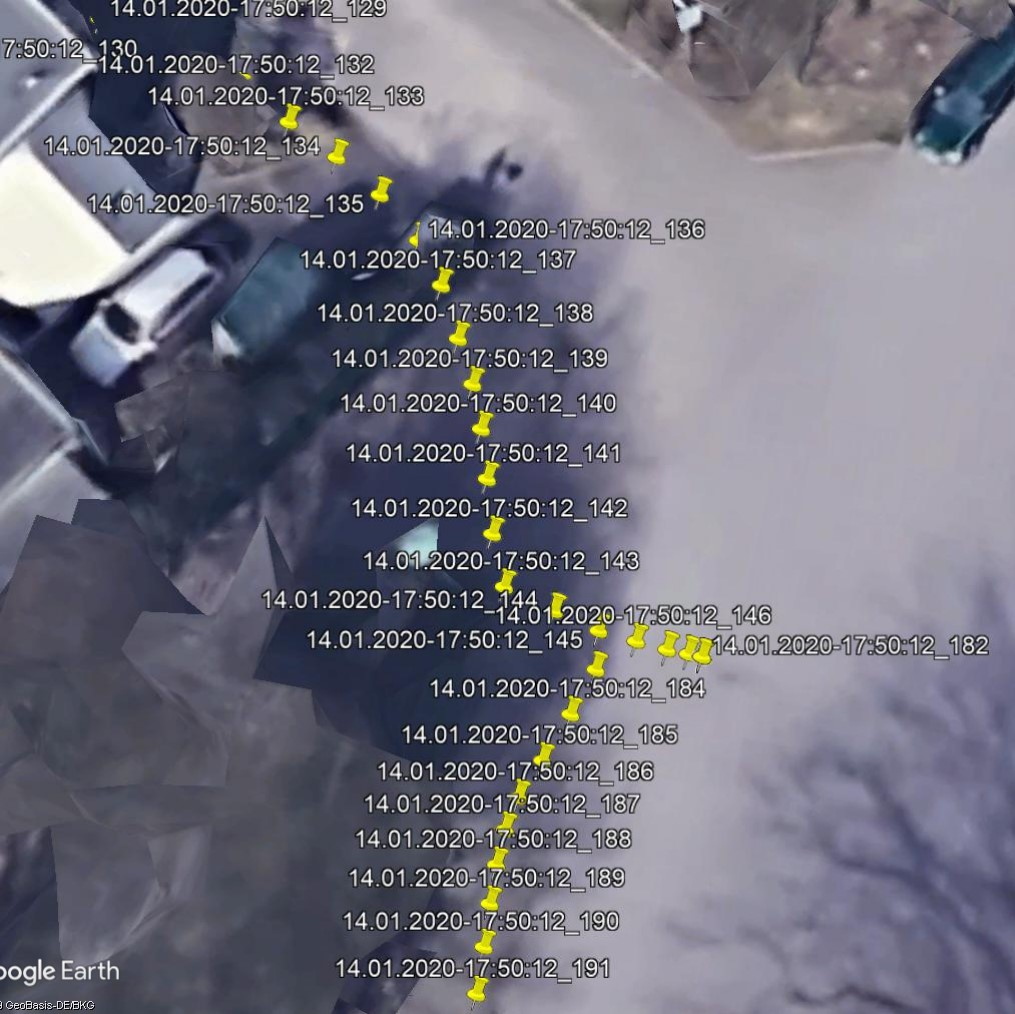
\includegraphics[width=0.8\textwidth]{Route1_abweichung_pause_1}
    \caption{Spitze 1.Pause}
    \label{fig:map}
\end{figure}
\begin{figure}[h!]
    \centering
    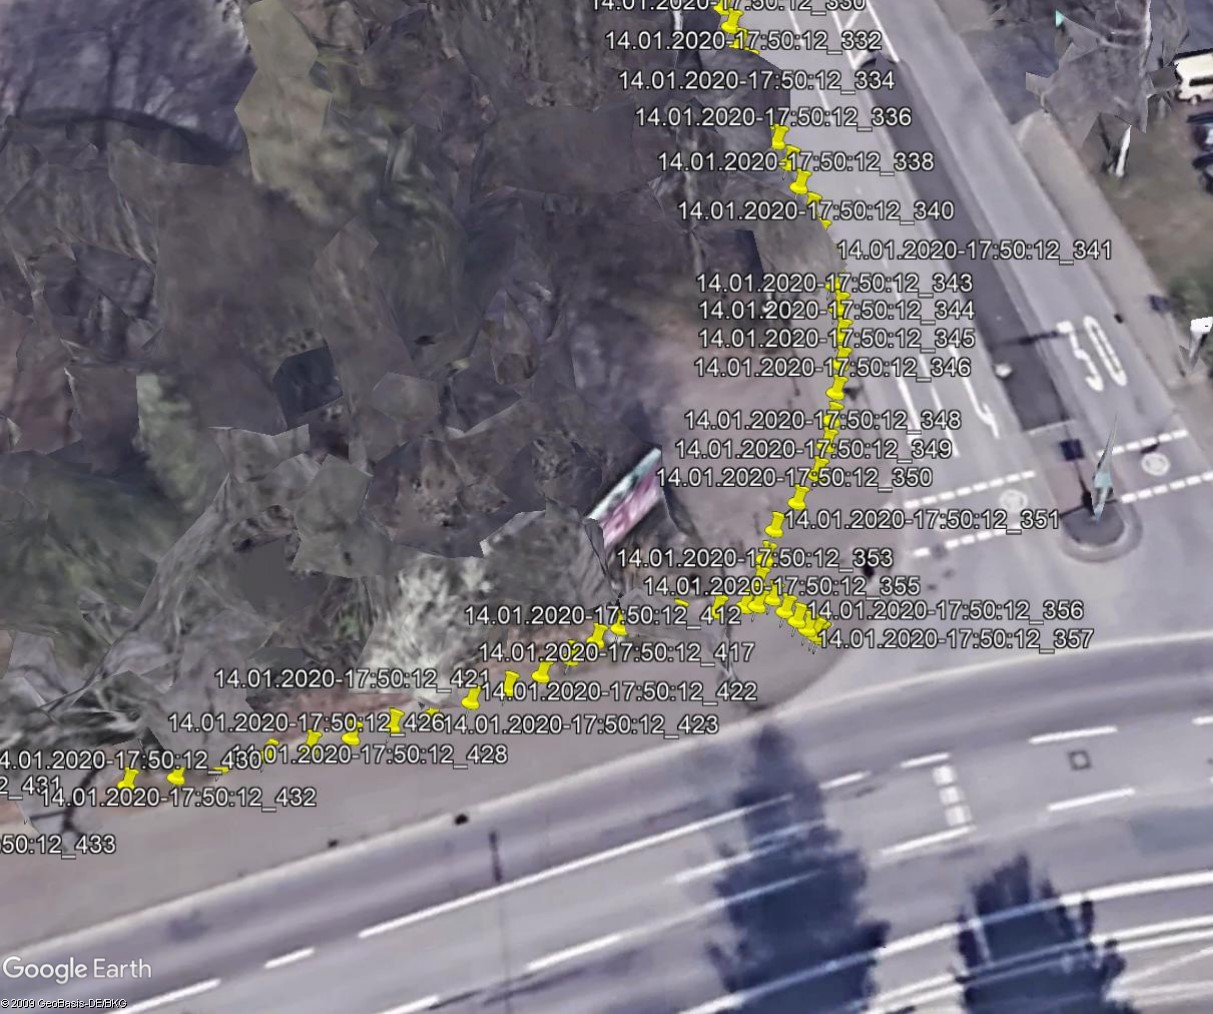
\includegraphics[width=0.8\textwidth]{Route1_abweichung_pause_2}
    \caption{Spitze 2.Pause}
    \label{fig:map}
\end{figure}

\begin{figure}[h!]
    \centering
    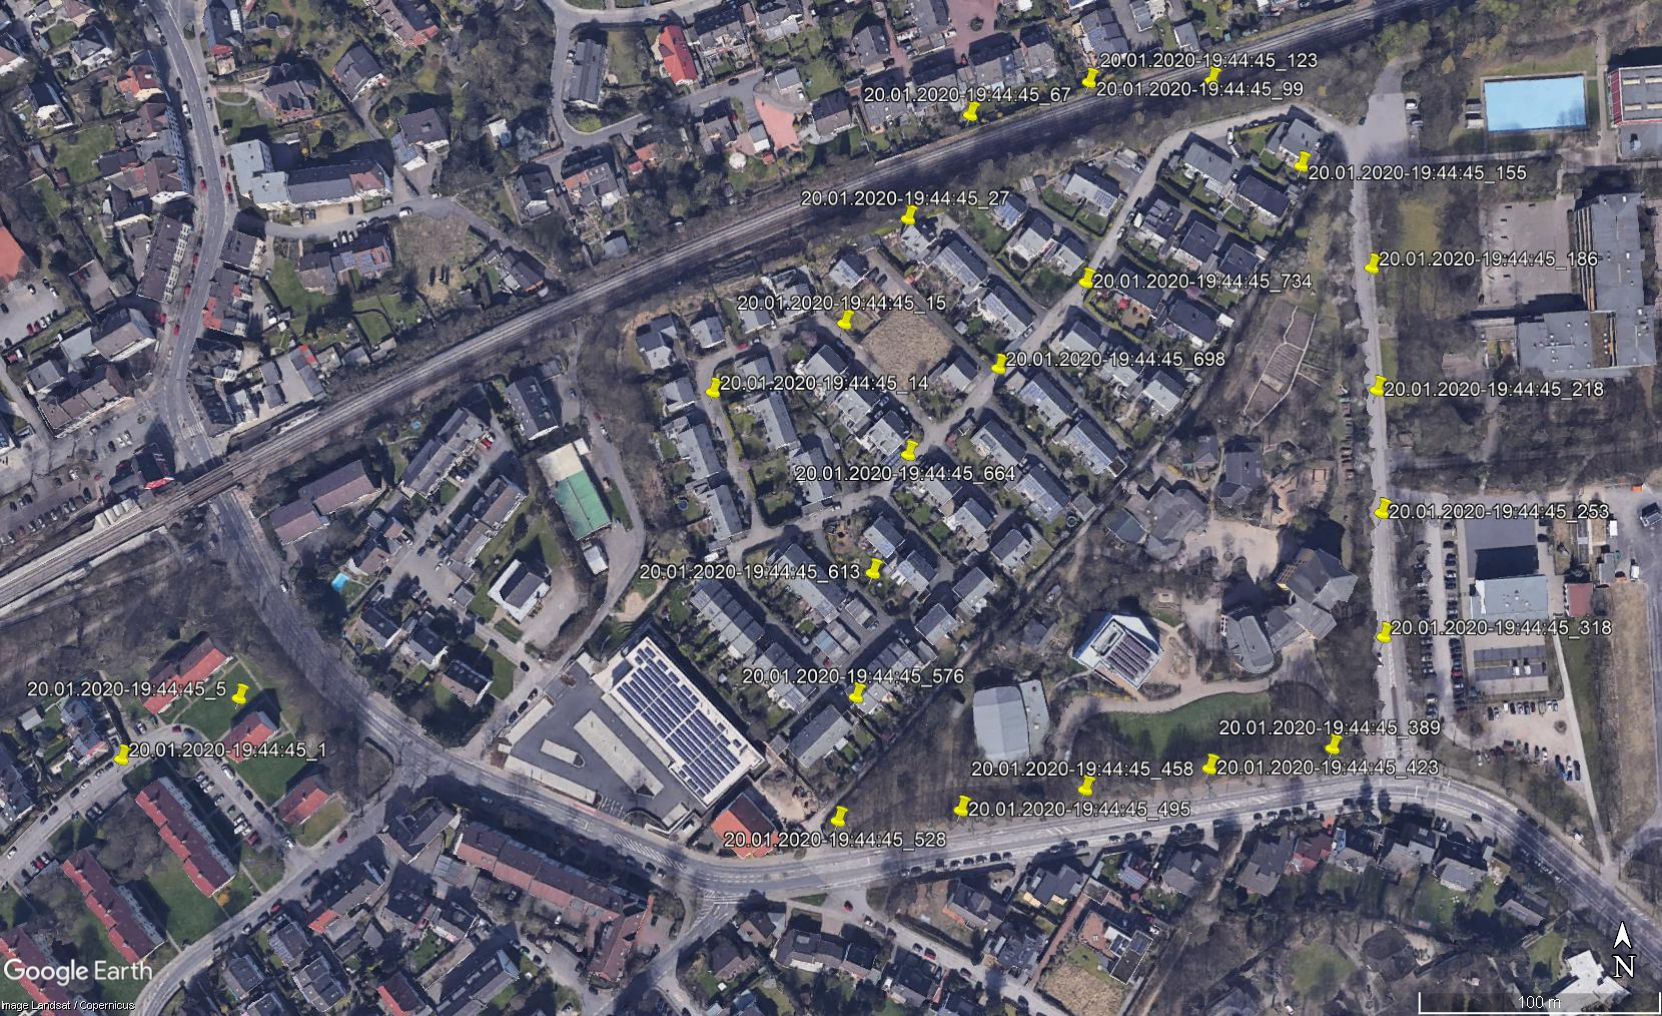
\includegraphics[width=0.8\textwidth]{Route2}
    \caption{Übersicht Fixes Messung 2}
    \label{fig:map}
\end{figure}

\begin{figure}[h!]
    \centering
    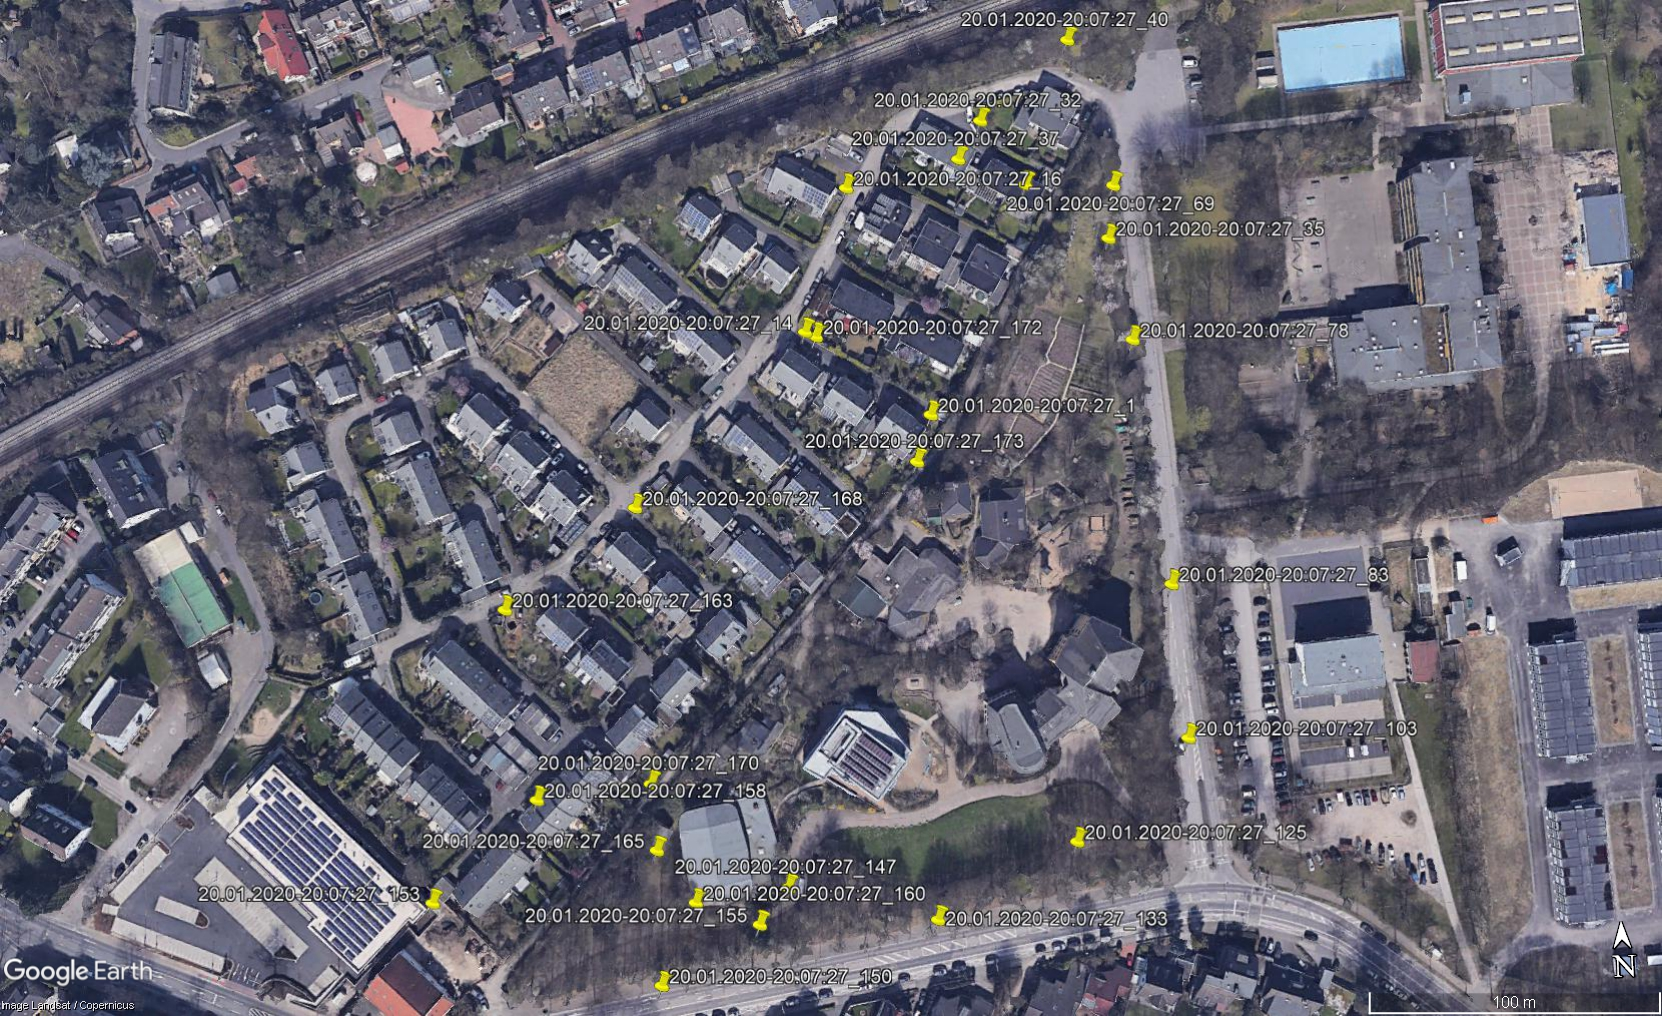
\includegraphics[width=0.8\textwidth]{Route3}
    \caption{Übersicht Fixes Messung 3}
    \label{fig:map}
\end{figure}

\begin{figure}[h!]
    \centering
    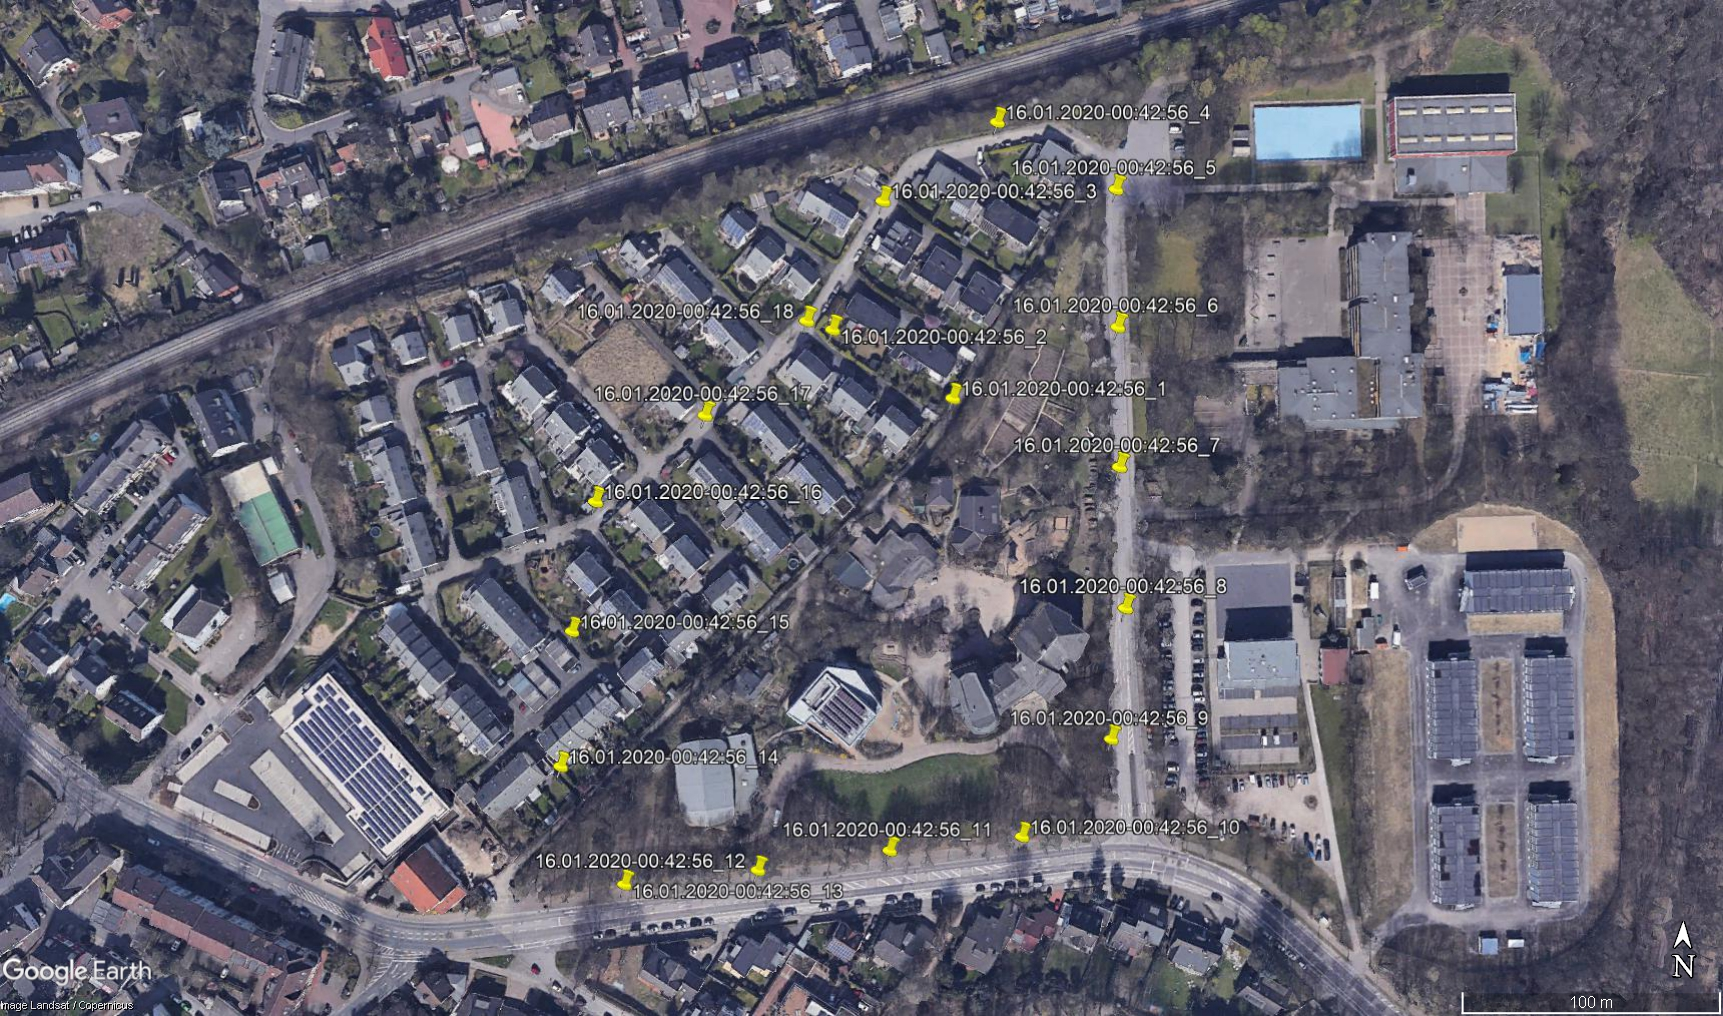
\includegraphics[width=0.8\textwidth]{Route4}
    \caption{Übersicht Fixes Messung4}
    \label{fig:map}
\end{figure}
	
\end{document}